% !TeX root = ../../formal_mordell_weil_rank_2026-07-30.tex
%
% GENERATED FILE -- do not edit by hand.
% Produced by Papers/figures/mordell_weil/make_figures.py
% Okabe--Ito colourblind-safe palette
\definecolor{clrP}{HTML}{0072B2}
\definecolor{clrQ}{HTML}{D55E00}
\definecolor{clrS}{HTML}{009E73}
\definecolor{clrD}{HTML}{CC79A7}
\definecolor{clrBand}{HTML}{56B4E9}
\definecolor{clrGrey}{HTML}{6E6E6E}

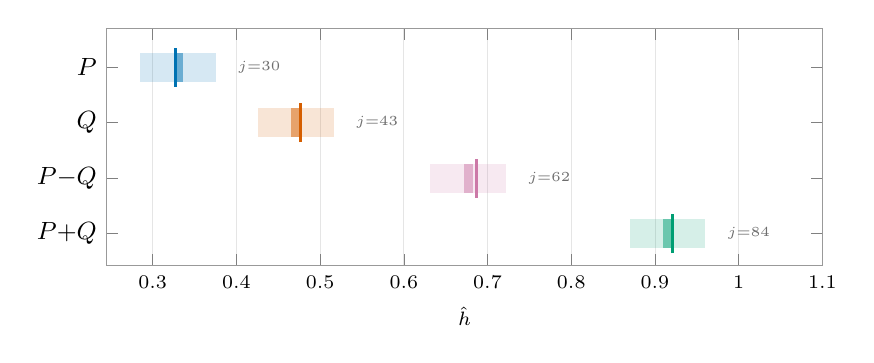
\begin{tikzpicture}
\begin{axis}[
  width=0.88\linewidth, height=4.6cm,
  xlabel={$\hat h$}, xmin=0.245, xmax=1.10,
  ymin=0.42, ymax=4.70,
  ytick={4,3,2,1}, yticklabels={$P$,$Q$,$P{-}Q$,$P{+}Q$},
  tick label style={font=\scriptsize}, label style={font=\scriptsize},
  y tick label style={font=\small},
  axis line style={clrGrey!70}, ymajorgrids=false,
  xmajorgrids, grid style={clrGrey!18, line width=0.3pt},
  xtick distance=0.1,
  clip=false,
]

\fill[clrP, fill opacity=0.16]
  (axis cs:0.285199,3.74) rectangle (axis cs:0.375457,4.26);
\fill[clrP, fill opacity=0.50]
  (axis cs:0.324913,3.74) rectangle (axis cs:0.335743,4.26);
\draw[clrP, line width=1.15pt]
  (axis cs:0.326999,3.65) -- (axis cs:0.326999,4.35);
\node[font=\tiny, color=clrGrey, anchor=west]
  at (axis cs:0.390457,4) {$j{=}30$};

\fill[clrQ, fill opacity=0.16]
  (axis cs:0.425995,2.74) rectangle (axis cs:0.516252,3.26);
\fill[clrQ, fill opacity=0.50]
  (axis cs:0.465708,2.74) rectangle (axis cs:0.476539,3.26);
\draw[clrQ, line width=1.15pt]
  (axis cs:0.476712,2.65) -- (axis cs:0.476712,3.35);
\node[font=\tiny, color=clrGrey, anchor=west]
  at (axis cs:0.531252,3) {$j{=}43$};

\fill[clrD, fill opacity=0.16]
  (axis cs:0.631773,1.74) rectangle (axis cs:0.722030,2.26);
\fill[clrD, fill opacity=0.50]
  (axis cs:0.671486,1.74) rectangle (axis cs:0.682317,2.26);
\draw[clrD, line width=1.15pt]
  (axis cs:0.686665,1.65) -- (axis cs:0.686665,2.35);
\node[font=\tiny, color=clrGrey, anchor=west]
  at (axis cs:0.737030,2) {$j{=}62$};

\fill[clrS, fill opacity=0.16]
  (axis cs:0.870042,0.74) rectangle (axis cs:0.960300,1.26);
\fill[clrS, fill opacity=0.50]
  (axis cs:0.909756,0.74) rectangle (axis cs:0.920586,1.26);
\draw[clrS, line width=1.15pt]
  (axis cs:0.920756,0.65) -- (axis cs:0.920756,1.35);
\node[font=\tiny, color=clrGrey, anchor=west]
  at (axis cs:0.975300,1) {$j{=}84$};

\end{axis}
\end{tikzpicture}
